\chapter{Conclusiones y trabajo futuro} \label{cap:capitulo8}

\section{Trabajo futuro}

Lamentablemente el proyecto no ha podido completarse al 100\% por falta de tiempo. La incertidumbre causada por un roadmap que no siempre estuvo claro, la gran inexperiencia en la materia y la dependencia de una infraestructura software y hardware que no siempre estuvo exenta de fallos han supuesto unos riesgos en el proyecto que finalmente han acabado materializándose. Sin embargo, sí que se ha conseguido realizar gran parte del camino, llegando a ver la meta final a tan solo unas pocas semanas más de trabajo (se estima que el proyecto se encuentra entorno al 90\% de completitud).

Principalmente ha faltado la realización de más pruebas sobre el software, para detectar errores y refinar el sistema. Todas las funcionalidades integradas en el proyecto se han sometido a una serie de pruebas que garantizar su funcionamiento, pero en aquellas partes relacionadas con el campo de la acústica es difícil como Ingeniero Informática dar por válido o no el funcionamiento.

Relacionado con esto está \textbf{el proceso de limitación}, del cuál no se ha podido realizar ningún test más allá de su correcta compilación, el \textbf{proceso de calibración} el cual se ha probado y parece funcionar correctamente pero no se sabe con seguridad por la inexperiencia en el campo.

% getData ???

Además de lo comentado hasta ahora, como trabajo futuro se propone lo siguiente:

\begin{enumerate}
	\item Proporcionar a la \glsname{API-REST} de una capa de seguridad mediante \glsname{OAuth2} \cite{oauth} o API tokens \cite{openapi-auth}.
	\subitem \noindent Actualmente la \glsname{API-REST} carece de seguridad en este sentido y es completamente abierta y pública a la red. Como el equipo se encuentra en fase de prototipo esto no es esencial de momento, pero sí que lo es para poder pasar a producción.

	\item Mejorar el manejo de la configuración (y posiblemente el de los ficheros de audio también) mediante el uso de una base de datos (relacional o no relacional).

	\item Simplificar el registro.
	\subitem El archivo de registro podría ser perfectamente un fichero con formato \acrshort{JSON} en el que cada una de las líneas representa un registro. De esta forma, su manejo y mantenimiento sería inmensamente más simple, y el programa \texttt{get-data} tan sólo tendría que consultar y devolver los registros solicitados, sin necesidad de darles formato.

	\item Diseño e implementación de un sistema que notifique a los servicios del limitador de los eventos que les interesen, como por ejemplo un despachador de eventos. Ver imagen \ref{fig:event-dispatcher}.
	\subitem \noindent Por ejemplo, notificar a los servicios si se modifica la configuración. Actualmente recargan la configuración cada 10 segundos.

	\item Continuar con el proceso de mejora y refactoring para arreglar los problemas mencionados en la sección \ref{sec:errores} respecto al código.

	\item Verificar el buen funcionamiento del equipo.

	\item Integrar el uso del \acrshort{LCD}, \acrshort{LED}s y Buzzer como parte del software principal.
	\subitem \noindent Actualmente estos elementos funcionan y pueden ser controlados mediante código, pero no hay ningún programa que los utilice, tan sólo los de prueba.

	\item Promocionar todos los programas que deben correr de forma ininterrumpida a servicios de \textbf{systemd}.
\end{enumerate}


\begin{figure}[h]
    \centering
    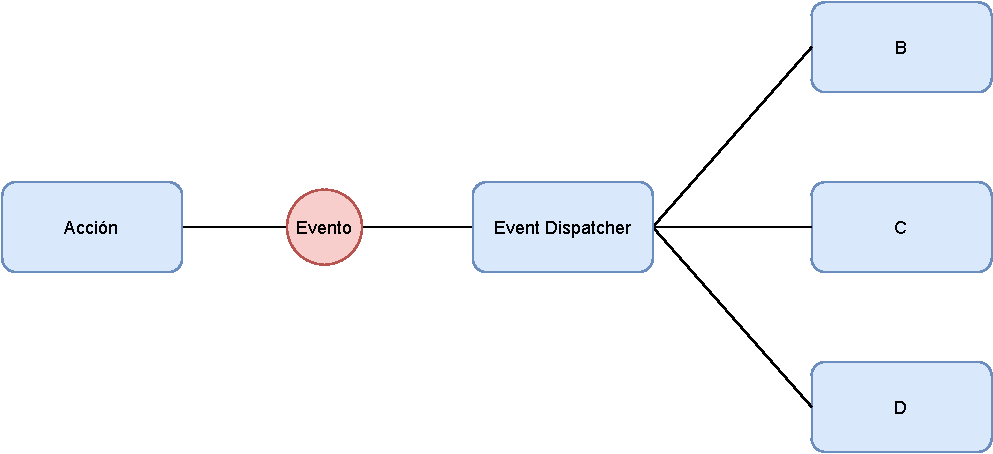
\includegraphics[width=0.75\textwidth]{figuras/event-dispatcher.pdf}
    \caption{Diagrama conceptual de un Despachador de Eventos.}
    \label{fig:event-dispatcher}
\end{figure}

\section{Conclusiones}

Como punto final a la realización de este Trabajo de Fin de Grado se procede a repasar cada uno de los objetivos del proyecto, indicando su grado de cumplimiento y cómo se han abordado.

Los resultados obtenidos en este proyecto han sido mayormente satisfactorios, ya que se han cumplido la gran mayoría de los objetivos y requisitos marcados y se han puesto en práctica los conocimientos adquiridos en durante la realización del Grado en Ingeniería Informática. De hecho, la naturaleza del proyecto, no sólo ha exigido el uso del conocimiento adquirido en varias áreas de la informática, sino que ha requerido el aprendizaje de metodologías y herramientas nuevas, tanto del área de la informática, como del área de la ingeniería y la electrónica. Además, se ha trabajado en un entorno plural en el que la cooperación y la comunicación entre los compañeros y compañeras para el alcance de los objetivos de éste, y de otros proyectos, ha tenido un papel determinante.

El objetivo principal casi ha quedado completado. Se dispone de un equipo capaz de registrar los niveles de presión acústica de emisión y recepción en el local donde se encuentra instalado. Esto se ha conseguido mediante el uso de un micrófono y transformaciones matemáticas, que quedan fuera del ámbito de este proyecto, para obtener un modelo acústico medido en decibelios a partir de la intensidad de la señal de entrada. La atenuación del sonido por el contrario no ha podido completarse debido a falta de tiempo, pero sí que se ha generado un diseño, una implementación (no probada) y funcionalidad para controlar el actuador, el PGA instalado en el hardware. Todas estas cuestiones han sido descritas a mayor nivel de detalle en el capítulo de \nameref{cap:capitulo5}.

El resto de objetivos y requisitos han sido completados, se han estudiado las necesidades de un sistema de estas características mediante el extenso proceso de ingeniería inversa que se ha realizado sobre los limitadores \acrshort{LM7} y \acrshort{LM9}, redactado en los capítulos \nameCref{cap:capitulo3_I}, \nameref{cap:capitulo3_II} y \nameref{cap:capitulo3_III}. De estas necesidades se han extraído los requisitos del sistema, descritos en el apartado \nameref{cap:capitulo2}. Como resultado también del proceso de ingeniería inversa, se ha estudiado si había elementos en estos sistemas que pudieran ser de utilidad en nuestro proyecto en el capítulo \nameref{cap:capitulo4}, y se ha diseñado e implementado el sistema requerido: capítulos \nameref{cap:capitulo5} y \nameref{cap:capitulo6}. Finalmente, se ha realizado una serie de pruebas para comprobar el buen funcionamiento del diseño propuesto y la implementación realizada, capítulo \nameref{cap:capitulo7}

El hecho de que en el momento de dar punto final al proyecto no se disponga de un equipo completamente operativo para entrar a producción no eclipsa todo el trabajo, esfuerzo y tiempo invertido en el proyecto. Todas las herramientas y piezas necesarias para su finalización están completamente disponibles llegados a este punto, por lo que llevar el producto a su estado final no debería implicar demasiado esfuerzo adicional. De hecho, todo el trabajo realizado durante este proyecto se traduce de forma directa en una sólida base sobre la que poder trabajar y continuar el desarrollo del producto, de forma que un un futuro pueda entrar al mercado.

A nivel personal, considero sin duda alguna que los mayores logros durante la realización de este proyecto ha sido el proporcionar una extensa documentación en la que se reflejan las necesidades de un sistema de estas características, su diseño y su funcionamiento, así como proporcionar un proyecto software con una estructura y un código inmensamente mejor en cuanto a calidad se refiere.

Como comentario final, decir que aunque ha sido una experiencia inesperadamente dura, y muchas veces frustrante, me doy por satisfecho con el titánico trabajo realizado y considero que finalizo este proyecto con más y mejores capacidades como profesional.